\documentclass[12pt,a4paper]{scrartcl} 
\usepackage[utf8]{inputenc}
\usepackage[english,russian]{babel}
\usepackage{indentfirst}
\usepackage{misccorr}
\usepackage{graphicx}
\usepackage{indentfirst}
\usepackage{amsmath}
\begin{document}
 \begin{titlepage}
  \begin{center}
   \large
   МИНИСТЕРСТВО НАУКИ И ВЫСШЕГО ОБРАЗОВАНИЯ РОССИЙСКОЙ ФЕДЕРАЦИИ
   
   Федеральное государственное бюджетное образовательное учреждение высшего образования
   
   \textbf{АДЫГЕЙСКИЙ ГОСУДАРСТВЕННЫЙ УНИВЕРСИТЕТ}
   \vspace{0.25cm}
   
   Инженерно-физический факультет
   
   Кафедра автоматизированных систем обработки информации и управления
   \vfill

   \vfill
   
   \textsc{Отчет по практике}\\[5mm]
   
   {\LARGE Верификация ГИА \textit{}}
   \bigskip
   
   1 курс, группа 1ИВТ-АСОИУ
  \end{center}
  \vfill
  
  \newlength{\ML}
  \settowidth{\ML}{«\underline{\hspace{0.7cm}}» \underline{\hspace{2cm}}}
  \hfill\begin{minipage}{0.5\textwidth}
   Выполнил:\\
   \underline{\hspace{\ML}} С.\,Р.~Александров\\
   «\underline{\hspace{0.7cm}}» \underline{\hspace{2cm}} 2024 г.
  \end{minipage}%
  \bigskip
  
  \hfill\begin{minipage}{0.5\textwidth}
   Руководитель:\\
   \underline{\hspace{\ML}} С.\,В.~Теплоухов\\
   «\underline{\hspace{0.7cm}}» \underline{\hspace{2cm}} 2024 г.
  \end{minipage}%
  \vfill
  
  \begin{center}
   Майкоп, 2024 г.
  \end{center}
 \end{titlepage}
 
% Содержание
\section{Введение}
\label{sec:intro}


\subsection{Формулировка цели}
Целью данной работы является верификация ГИА.

\subsubsection{Теория}
Бланки участников ГИА из всех пунктов проведения экзамена проходят сканирование после обработки машиночитаемых форм. По завершении работы оператор сравнивает результаты сканирования, а также проверяет качество сканирования. Этот процесс позволяет убедиться в корректности и полноте сканирования.\\
\\
Сканирование и распознавание бланков:

\begin{itemize}
    \item Оптическое сканирование: С помощью сканера создается цифровое изображение бланка. \\
    \item Предварительная обработка изображений: Включает выравнивание, удаление шумов и улучшение качества изображения.\\
    \item Оптическое распознавание символов (OCR): Программное обеспечение анализирует изображение и преобразует текстовые и графические элементы в машинно-читаемый формат.\\
    \item Проверка данных: Полученные данные проверяются на наличие ошибок, таких как неправильное распознавание символов или неполное сканирование\\
\end{itemize}

Методы и алгоритмы OCR:\\
OCR (Optical Character Recognition) использует различные алгоритмы для распознавания текста:

\begin{itemize}
    \item Шаблонное распознавание: Сравнение отсканированных символов с заранее заданными шаблонами.\\
    \item Функциональное распознавание: Анализ формы и структуры символов.\\
    \item Методы машинного обучения и нейронных сетей: Использование обученных моделей для улучшения точности распознавания.\\
\end{itemize}


\section{Ход работы}
\sloppy
Ознакомился с оборудованием и программным обеспечением:
\begin{itemize}
    \item Прошел инструктаж по технике безопасности и правилам работы с оборудованием. \\
    \item Ознакомился с установленным программным обеспечением для проверки сканированных бланков (например, ABBYY FineReader, специализированное ПО для обработки ГИА)..\\
\end{itemize}
Анализ и проверка распознанных данных:
\begin{itemize}
    \item Визуально сравнил отсканированные изображения с оригинальными бумажными бланками, если это возможно. \\
    \item Проверил корректность распознавания символов и текста:\\
    \begin{itemize}
    \item Обратил внимание на правильность распознавания фамилий, имен, номеров участников и других важных данных.
    \item Проверил правильность распознавания отметок в полях ответов.
    \end{itemize}
\end{itemize}
Исправление ошибок:
\begin{itemize}
    \item Внес исправления вручную в случае обнаружения ошибок:\\
    \begin{itemize}
    \item Корректировка неправильно распознанных символов.
    \item Исправление неверно распознанных или пропущенных данных.
    \end{itemize}
\end{itemize}
Сохранение изменений:
\begin{itemize}
    \item Сохранил исправленные данные.\\

\begin{figure}[h]
\centering
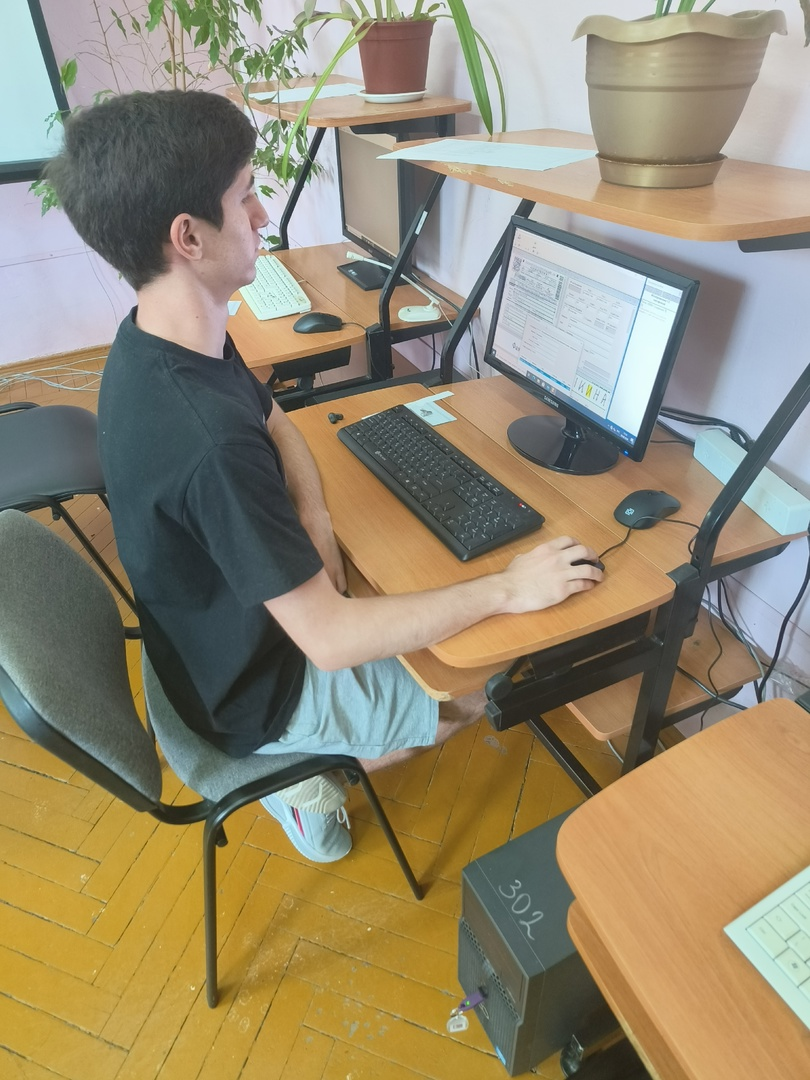
\includegraphics[width=0.8\linewidth]{image.png}
\caption{Процесс верификации}
\label{fig:mpr}
\end{figure}
\end{itemize}

\section{Вывод}
Таким образом, основная задача заключалась в тщательной проверке корректности отсканированных бланков ГИА и внесении необходимых исправлений для обеспечения точности данных.


\end{document}